\documentclass[12pt]{beamer}

\usepackage{amsmath}
\usepackage{amssymb}
\usepackage{graphics, subfigure}
%\pagestyle{empty}
\usepackage{slashbox}

\usepackage{color}
\newcommand{\hilight}[1]{\colorbox{yellow}{#1}}
%\usepackage{soul}


\usetheme[secheader]{Madrid}
\usefonttheme[stillsansserifsmall]{serif}
\usefonttheme[onlylarge]{structurebold}
\usecolortheme[RGB={10,120,100}]{structure}
\setbeamertemplate{navigation symbols}{}

%\input{defs}


\author[]{%
  Chen Greif, Dan Li, Dominik Sch\"{o}tzau, \underline{Michael Wathen} \\
  The University of British Columbia, Vancouver, Canada }
%\title%[\hfill\insertframenumber/\inserttotalframenumber]
\title[]{Block Preconditioners for an Incompressible Magnetohydrodynamics Problem}
\date[]{17\textsuperscript{th} June 2015 \\ Preconditioning 2015 \\ Eindhoven, NL
}


%\institute[]{University of British Columbia, Vancouver, Canada}

\definecolor{darkgreen}{rgb}{0,0.5,0}
\definecolor{darkyellow}{rgb}{.8,.6,.04}
\newcommand{\gr}[1]{\textcolor{darkgreen} {#1}}
\newcommand{\wh}[1]{\textcolor{white}     {#1}}
\newcommand{\dy}[1]{\textcolor{darkyellow}{#1}}
\newcommand{\yb}[1]{\colorbox {yellow}    {#1}}
\newcommand{\re}[1]{{\textcolor{red}       {#1}}}
\newcommand{\bl}[1]{{\textcolor{blue}{#1}}}

\newcommand{\RE}[1]{{\bf\textcolor{red}       {#1}}}
\newcommand{\GR}[1]{{\bf\textcolor{darkgreen} {#1}}}
\newcommand{\DY}[1]{{\bf\textcolor{darkyellow}{#1}}}
\newcommand{\BL}[1]{{\bf\textcolor{blue}{#1}}}
\newcommand{\ssec}[1]{{\bf #1}}
\newcommand{\rsec}[1]{{\bf\color{red}       #1}}
\newcommand{\bsec}[1]{{\bf\color{blue}      #1}}
\newcommand{\gsec}[1]{{\bf\color{darkgreen} #1}}
\newcommand{\dom}{\mbox{\sf dom}}

\newcommand{\curl}{\ensuremath{\nabla\times\,}}
\renewcommand{\div}{\nabla\cdot\,}
\newcommand{\grad}{\ensuremath{\nabla}}



\newcommand{\R}{\mathbb{R}}
\newcommand{\minim}{\mathop{\mathrm{minimize}}}
\newcommand{\minimize}[1]{\displaystyle\minim_{#1}}
\newcommand{\maxim}{\mathop{\mathrm{maximize}}}
\newcommand{\maximize}[1]{\displaystyle\maxim_{#1}}
\newcommand{\st}{\mathop{\mathrm{subject\ to}}}
\newcommand{\Null}{\mathop{\mathrm{Null}}}
\newcommand{\A}{\mathcal{A}}
\newcommand{\I}{\mathcal{I}}

\begin{document}

\begin{frame}
  \titlepage
\end{frame}



\title{MHD}
% \section{Introduction}

% \begin{frame}

% \frametitle{Continuous and Discrete Maxwell's equations}
% \begin{tabular}{lrrrr}
% \hline
% {} &  Grid size &      DoF &  $\#$ iters &  Soln Time \\
% \hline
% 0 &       $   2^3$ &       81 &        1 &   4.25e-04 \\
% 1 &       $   4^3$ &      375 &        3 &   6.03e-04 \\
% 2 &       $   8^3$ &     2187 &        5 &   2.53e-03 \\
% 3 &      $  16^3$ &    14739 &        5 &   1.96e-02 \\
% 4 &      $  32^3$ &   107811 &        6 &   2.24e-01 \\
% 5 &      $  64^3$ &   823875 &        6 &   2.28e+00 \\
% 6 &     $ 128^3$ &  6440067 &        6 &   2.09e+01 \\
% \hline
% \end{tabular}

% \end{frame}


% \section{Overview}
% \begin{frame}
% \begin{center}
%   Overview
% \end{center}

% \begin{itemize}
%   \item Problem background: Setup, ...
%   \item
% \end{itemize}

% \end{frame}

\section{Problem background}
\begin{frame}{Problem background}

\begin{itemize}
  \item MHD models electrically conductive fluids (such as liquid metals, plasma, salt water, etc) in an electic field
  \pause
  \item Applications: electromagnetic pumping, aluminium electrolysis, the Earth's molten core and solar flares
  \pause
  \item MHD couples electromagnetism (governed by Maxwell's equations) and fluid dynamics (governed by the Navier-Stokes equations)
  \pause
  \begin{itemize}
    \item Movement of the conductive material that induces and modifies any existing electromagnetic field
    \pause
    \item Magnetic and electric fields generate a mechanical force on the fluid
  \end{itemize}
\end{itemize}

\end{frame}
\section{MHD}
\begin{frame}{MHD model: coupled Navier-Stokes and Maxwell's equations}

\begin{subequations} \nonumber
% \label{eq:mhd}
\re{\begin{alignat}2
% \label{eq:mhd1}
 - \nu  \, \Delta{u} + ({u} \cdot \nabla)
{u}+\nabla p  {\only<2>{\color{blue}}- \kappa\,
(\nabla\times{b})\times{b}} &= {f} & \qquad &\mbox{in $\Omega$},\\[.1cm]
% \label{eq:mhd2}
\nabla\cdot{u} &= 0 & \qquad &\mbox{in $\Omega$},\\[.1cm]
% \label{eq:mhd3}
\kappa\nu_m  \, \nabla\times( \nabla\times {b})
+ \nabla r
{\only<2>{\color{blue}}- \kappa \, \nabla\times({u}\times {b})}  &= {g} & \qquad &\mbox{in $\Omega$},\\[.1cm]
% \label{eq:mhd4}
 \nabla\cdot{b} &= 0 & \qquad &\mbox{in $\Omega$},
\end{alignat}}
\end{subequations}
with appropriate boundary conditions
\pause
\begin{itemize}
  \item ${\color{blue}(\nabla\times{b})\times{b}}$:  Lorentz force accelerates the fluid particles in the direction normal to
 the electric and magnetic fields

  \item ${\color{blue} \nabla\times({u}\times {b})}$: electromotive force modifying the magnetic field
\end{itemize}
\end{frame}




\subsection{Navier-Stokes equations} % (fold)

\begin{frame}
\frametitle{Steady-state Navier-Stokes equations}
Incompressible Navier-Stokes Equations:

\begin{subequations}\nonumber
  \re{\begin{alignat}2
    - \nu  \, \Delta{u}+({u} \cdot \nabla){u} +\nabla p &= {f} & \qquad &\mbox{in $\Omega$},\\[.1cm]
    \nabla\cdot{u} &= 0 & \qquad &\mbox{in $\Omega$},\\[.1cm]
    u &= u_D & \qquad &\mbox{on $\partial \Omega$}
    \end{alignat}}
\end{subequations}%

\noindent where $\re{u}$ is the fluids velocity; $\re{p}$ is the fluids pressure; $\re{f}$ is the body force acting on the fluid and $\re{\nu}$ the kinematic viscosity


\end{frame}


\begin{frame}{Steady-state Navier-Stokes equations}

Corresponding linear system:
$$\re{\mathcal{K}_{\rm NS}=\begin{pmatrix}
A+0 & B^T \\
B & 0
\end{pmatrix}
\begin{pmatrix}
u\\p
\end{pmatrix}=
\begin{pmatrix}
f \\ 0
\end{pmatrix}
}$$
where $\re{A\in\mathbb{R}^{n_u\times n_u}}$ is the discrete Laplacian; $\re{O\in\mathbb{R}^{n_u\times n_u}}$ is the discrete convection operator and $\re{B\in\mathbb{R}^{m_u\times n_u}}$ is a discrete divergence operator with full row rank.

\vspace{2mm}

\bl{Note}: due to convection term the linear system is non-symmetric

\vspace{2mm}

For an extensive discussion of preconditioners we refer to \gr{Elman, Silvester and Wathen 2014}.

\end{frame}



\subsection{Maxwell's Equations} % (fold)
\begin{frame}{Time-Harmonic Maxwell in mixed form}
Maxwell operator in mixed form:
\begin{subequations}\nonumber
  \re{\begin{alignat}2
    \nabla\times( \nabla\times {b}) -k^2 b +\grad r &= {g} & \qquad &\mbox{in $\Omega$},\\[.1cm]
    \nabla\cdot{b} &= 0 & \qquad &\mbox{in $\Omega$},\\[.1cm]
    b \times n &= b_D & \qquad &\mbox{on $\partial \Omega$},\\[.1cm]
    r &= 0& \qquad &\mbox{on $\partial \Omega$},
    \end{alignat}}\\[.1cm]
\end{subequations}
where $\re{b}$ is the magnetic vector field, $\re{r}$ is a scalar multiplier and $\re{k}$ is the wave number

\vspace{2mm}

\bl{Note:} for the MHD system $\re{k = 0}$

\end{frame}

\begin{frame}{Time-Harmonic Maxwell in mixed form}
Corresponding linear system:
\begin{equation}
\nonumber
\re{\begin{pmatrix}
M-k^2X & D^T \\
D & 0
\end{pmatrix}
\begin{pmatrix}
b \\
r
\end{pmatrix}
=
\begin{pmatrix}
g \\
0
\end{pmatrix}},
\end{equation}
where $\re{M\in\mathbb{R}^{n_b\times n_b}}$ is the discrete curl-curl operator; $\re{X\in\mathbb{R}^{n_b\times n_b}}$ the discrete mass matrix; $\re{D\in\mathbb{R}^{m_b\times n_b}}$ the discrete divergence operator

\vspace{2mm}

\bl{Note:} $\re{M}$ is semidefinite with nullity $\re{m_b}$

\vspace{2mm}

A significant amount of literature on time-harmonic Maxwell: notably for us, work of \gr{Hiptmair \& Xu 2007} for solving shifted curl-curl equations in a fully scalable fashion



\end{frame}



\section{Discretisation}
\begin{frame}{Discretisation}

\begin{itemize}
  \item Finite element discretisation based on the formulation in \gr{Sch{\"o}tzau 2004}
  \item Fluid variables: Mini element (P1+B3)/P1
  \item Magnetic variables: mixed {N\'{e}d\'{e}lec} element approximation N1/P1
  \item {N\'{e}d\'{e}lec} elements capture solutions correctly on non-convex domains
\end{itemize}

\begin{figure}[h]
    \begin{center}$
    \begin{array}{ccc}
    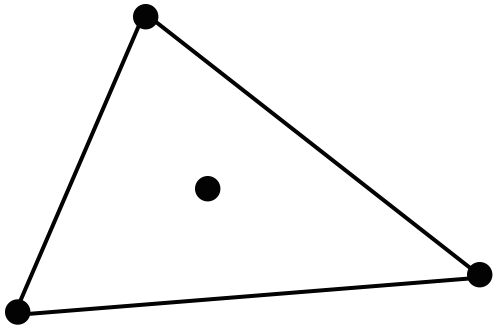
\includegraphics[width=30mm]{figures/bubble}& \quad &
    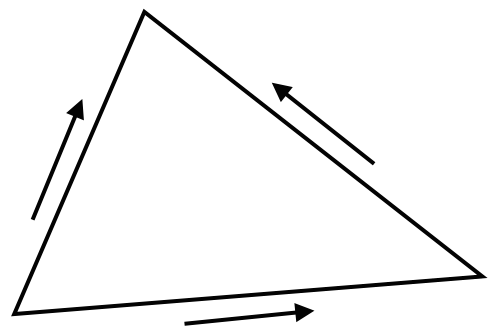
\includegraphics[width=30mm]{figures/nedelec}
    \end{array}$
    \end{center}
    \caption{Bubble element and {N\'{e}d\'{e}lec} element}
    \label{pics:blablabla}
\end{figure}

\end{frame}

\begin{frame}
Discretised and linearised MHD model:
\begin{equation}
\nonumber %\mathcal{K} x \equiv
\re{\left(
\begin{array}{cccc}
A+O(u) & B^T & C(b)^T & 0\\
B & 0 & 0 & 0 \\
-C(b) & 0 & M & D^T\\
0 & 0 & D & 0
\end{array}
\right)
\,
\left(
\begin{array}{c}
\delta u\\
\delta p\\
\delta b\\
\delta r
\end{array}
\right)  =
\begin{pmatrix}
r_u \\
r_p\\
r_b\\
r_r
\end{pmatrix},}
\end{equation}
with
\begin{equation}\nonumber
\re{\begin{array}{rl}
r_u &= f- Au -O(u) u - C(b)^T b- B^T p,\\
r_p &=-B u,\\
r_b &=g-Mu+C(b)b-D^T r,\\
r_r &=-D b.
\end{array}}
\end{equation}
$\re{C}$:~coupling terms

\vspace{2mm}
\pause
In some cases, it is possible to decouple
\begin{itemize}
\item Magnetic Decoupling (MD): if the coupling term is not large, just dump it and solve a block diagonal system
\item Complete Decoupling (CD): if convection is small, then dump convective term and obtain symmetry
\end{itemize}

  \end{frame}

\begin{frame}{A Few Comments}
\begin{itemize}
    \item Little has been done with respect to a preconditioned iterative solution method
    \item   \gr{Phillips, Elman, Cyr, Shadid, and Pawlowski 2014}: block preconditioners for an exact penalty formulation, using nodal elements; resulting system is block 3-by-3
    \item Results show good scalability with respect to the mesh
    \item Our formulation: {N\'{e}d\'{e}lec} (edge) elements, giving rise to a richer finite element space, 4-by-4 system, but with a different set of challenges
\end{itemize}


\end{frame}



\section{Preconditioning}


\begin{frame}{Ideal preconditioning}

Non-singular $(1,1)$ block (as in Navier-Stokes)
\begin{equation}\nonumber
\re{\mathcal{K} = \begin{pmatrix}
F & B^T \\
B & 0
\end{pmatrix}; \quad
\mathcal{P}=\begin{pmatrix}
F & B^T\\
0 & B F^{-1} B^T
\end{pmatrix}}
\end{equation}
\gr{Murphy, Golub \& Wathen 2000} showed exactly two eigenvalues:~$\pm 1$ %and $\nicefrac{1}{2}\pm \nicefrac{\sqrt{5}}{2}$

\vspace{5mm}
\pause
$\re{F}$ singular with nullity $\re{m}$ (as in time-harmonic Maxwell)

\begin{equation}\nonumber
\re{\mathcal{K} = \begin{pmatrix}
F & B^T \\
B & 0
\end{pmatrix}; \quad
\mathcal{P}=\begin{pmatrix}
F+B^T W^{-1} B & 0 \\
0 & W
\end{pmatrix}}, \ \mbox{where $\re{W}$ is SPD}
\end{equation}
\gr{Greif \& Sch{\"o}tzau 2006} showed exactly two eigenvalues: $\pm 1$

\end{frame}

\begin{frame}{Navier-Stokes subproblem}

$$\re{\mathcal{K}_{\rm NS}=\begin{pmatrix}
F & B^T \\
B & 0
\end{pmatrix}}$$
where $\re{F=A+O}$ is the discrete convection diffusion operator. Shown in \gr{Elman, Silvester \& Wathen 2014} that
$$\re{\mathcal{P}_{\rm NS}=\left(\begin{array}{cc}
F & B^T \\
0 & S
\end{array}\right)}, \quad \re{S =A_p F_p^{-1}Q_p}$$
is a good approximation to the Schur complement preconditioner. $\re{A_p}$:~pressure space Laplacian, $\re{F_p}$:~pressure space convection-diffusion operator, $\re{Q_p}$:~pressure space mass matrix
\end{frame}


\begin{frame}{Maxwell subproblem}
$$\re{\mathcal{K}_{\rm NS}=\begin{pmatrix}
M & B^T \\
B & 0
\end{pmatrix}}$$
\bl{Note:} M is highly rank deficient.

\gr{Greif \& Sch{\"o}tzau 2007} show that $\re{L}$ (scalar Laplacian) is the appropriate choice (from an inf-sup stability point of view)
$$\re{\mathcal{P}_{\rm iM}=\left(\begin{array}{cc}
M+B^T L^{-1} B & 0 \\
0 & L
\end{array}\right)}$$
\pause
Practical preconditioner:
$$\re{\mathcal{P}_{\rm M}=\left(\begin{array}{cc}
M+X & 0 \\
0 & L
\end{array}\right)}$$
where $\re{X}$ vector mass matrix is spectrally equivalent to $\re{B^T L^{-1} B}$
\end{frame}


\begin{frame}{MHD problem}
  Combining the Navier-Stokes and Maxwell preconditioners
  $$\re{\mathcal{P}_{\rm MH} =
  \left(
  \begin{array}{cccc}
  F  & B^T & C^T & 0\\
  0 & -{S} & 0 & 0 \\
  -C & 0 & M+X & 0\\
  0 & 0 & 0 & L
  \end{array}
  \right)}$$

\vspace{2mm}

\bl{Note:} $\re{{\mathcal{P}_{\rm MH}}}$ remains challenging to solve due to coupling terms. Schur complement approximation for velocity-magnetic unknowns

$$\re{\mathcal{P}_{\rm schurMH} =
\left(
\begin{array}{cccc}
F  + M_C & B^T & C^T & 0\\
0 & -{S} & 0 & 0 \\
0 & 0 & M+X & 0\\
0 & 0 & 0 & L
\end{array}
\right)}$$
where $\re{M_C = C^T (M + X)^{-1}C}$
\end{frame}


\begin{frame}{Spectral analysis (ideal preconditioner)}

\bl{Note:} using $\re{X = B^T L^{-1} B}$ for eigenvalue analysis

\begin{theorem}
\label{thm:mhd_outer_ideal}
The matrix $\re{\mathcal{P}_{\rm MH}^{-1} \mathcal{K}_{\rm MH} }$ has an eigenvalue $\re{\lambda = 1}$ with algebraic multiplicity of (at least) $\re{n_u + n_b}$ and an eigenvalue $\re{\lambda = -1}$ with  algebraic multiplicity of (at least) $\re{m_b}$.
\end{theorem}

\begin{theorem}
\label{thm:mhd_outer_schur}
The matrix $\re{\mathcal{P}_{\rm schurMH}^{-1} \mathcal{K}_{\rm MH}} $ has an eigenvalue $\re{\lambda = 1}$ with algebraic multiplicity of (at least) $\re{n_b+n_c}$ where $\re{n_c}$ is the dimension of the nullspace of $\re{C}$ and an eigenvalue $\re{\lambda = -1}$ with  algebraic multiplicity of (at least) $\re{m_b}$.
\end{theorem}
\end{frame}

\begin{frame}{Eigenvalue distribution}

\begin{figure}[h]
    \begin{center}
    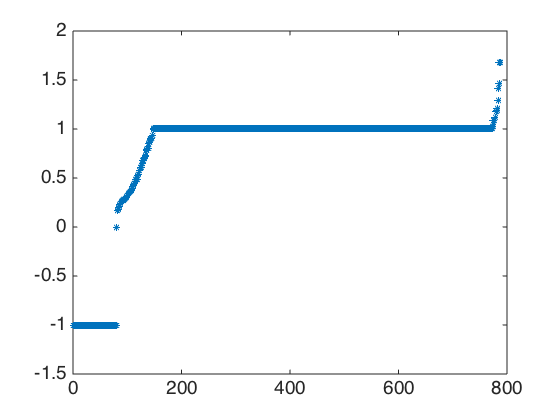
\includegraphics[width=80mm]{figures/Eigen}

    \caption{Real part of eigenvalues of preconditioned matrix~$\re{\mathcal{P}_{\rm schurMH}^{-1} \mathcal{K}_{\rm MH}}$ }
    \end{center}
\end{figure}




\end{frame}


\begin{frame}{Approximation for $\re{M_C}$}

Inspired by \gr{Phillips, Elman, Cyr, Shadid \& Pawlowski 2014}, we approximate $\re{M_C}$ by
$$\re{{M_C}\approx Q_s = {\kappa}{\nu_m}^{-1} {b} \times ({u}\times{b})}$$



\vspace{-4mm}


\begin{figure}[h]
    \begin{center}
    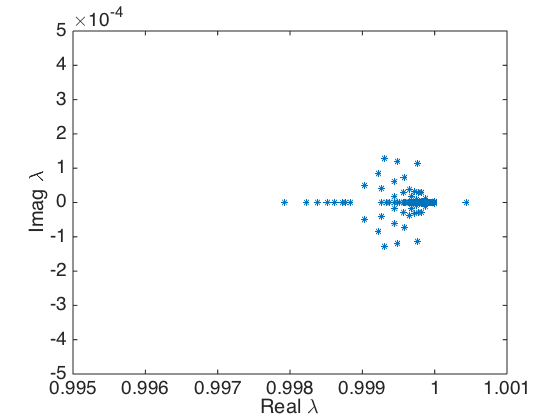
\includegraphics[width=65mm]{figures/mass}
    \end{center}
    \caption{Eigenvalues of preconditioned matrix $\re{(F+Q_S)^{-1}(F+M_C)}$ }
    \label{pics:blablabla}
\end{figure}

\end{frame}


\section{Numerical results}

\begin{frame}{Numerical software}

\begin{itemize}
  \item Finite element software \re{\tt FEniCS}:
  \begin{itemize}
    \item \re{\tt DOLFIN} problem-solving interface
    \item \re{\tt FFC} compiler for finite element variational forms
    \item \re{\tt FIAT}  finite element  tabulator
    \item \re{\tt Instant} just-in-time compiler
    \item \re{\tt UFC}  the code generator
    \item \re{\tt UFL} form language
  \end{itemize}
  \item Linear algebra software:
  \begin{itemize}
    \item \re{\tt PETSc} linear algebra wrapper features
    \item \re{\tt HYPRE} as a multigrid solver
    \item \re{\tt MUMPS} sparse direct solver
  \end{itemize}
\end{itemize}
\end{frame}

\begin{frame}{2D: smooth solution}
\begin{table} \footnotesize

\centering
\begin{tabular}{ccccccccccc}
\hline
 l &       DoF &  Average solve &  Total time &  Non-linear  & Average   \\
 & & Time & &its & its\\
\hline
  3 &       788 &       0.03 &           0.3 & 5 &     16.0 \\
  4 &      2,980 &       0.08 &           1.0 & 6 &     17.5 \\
  5 &     11,588 &       0.28 &           3.4 & 6 &     19.3 \\
  6 &     45,700 &       1.06 &          11.0 & 5 &     20.6 \\
  7 &    181,508 &       4.70 &          46.5 & 5 &     21.0 \\
  8 &    723,460 &      19.95 &         192.1 & 5 &     21.8 \\
  9 &   2,888,708 &      98.91 &         868.9 & 5 &     22.4 \\
 10 &  11,544,580 &     482.86 &        5794.1 & 5 &     24.2 \\
\hline
\end{tabular}
\caption{Number of nonlinear iterations and number of iterations to solve the MHD system with Tol = 1e-4, $\kappa$ = 1, $\nu$ = 1 and $\nu_m$ = 10}
\label{tab:MaxEigenvalues}
\end{table}

\end{frame}

\begin{frame}{Large scale 3D}
\begin{itemize}
\item Current goal: construct a high order (Taylor-Hood/{N\'{e}d\'{e}lec}) FE discretisation
\item This provides an accurate scheme and avoids stabilisation issues that are prevalent in lower order formulations.
\item Work in progress: implement with direct solvers, working on implementing the Hiptmair-Xu AMG preconditioning scheme.
\end{itemize}


\begin{table} \footnotesize
\centering
\begin{tabular}{lrrrrrll}
\hline
 l &       DoF &   Non-linear its  & Average its  \\
\hline
1 &     963 &                  3 &         19.7 \\
2 &    5,977 &                  3 &         25.3 \\
3 &   41,805 &                  3 &         26.7 \\
4 &  312,085 &                  3 &         27.0 \\
\hline
\end{tabular}
\caption{Number of nonlinear iterations and number of iterations to solve the MHD system with Tol = 1e-4, $\kappa$ = 1, $\nu$ = 1 and $\nu_m$ = 10}
\end{table}
\end{frame}

% \begin{frame}
% \begin{equation} \nonumber
%     \begin{aligned}
%       \re{  -\nu \Delta \vec u+ \nabla p} \ & \re{= \vec f} \\
%          \re{ \div \vec u   } \ & \re{= 0 }\\
%         % \vec u &= \vec 0 \ \ \ \mbox{on } \partial\Omega}
%     \end{aligned} \ \ \ \ \  \mbox{in } \Omega \hspace{24mm}
% \end{equation}
% \vspace{-3mm}
% \begin{equation} \nonumber
% \mbox{\hspace{-1.5mm}} \re{\vec u = \vec g} \ \ \ \ \ \ \mbox{on } \partial\Omega
% \end{equation}

% Viscosity $ \re{\nu}$, velocity $ \re{\vec u}$ and pressure $ \re{p}$

% \end{frame}

% \begin{frame}

% \frametitle{Stokes}

% $$ \re{\mathcal{K} = \begin{bmatrix}
% A & B^{\mbox{\tiny{T}}}\\
% B & 0\\
% \end{bmatrix} \hspace{15mm}
% \mathcal{M} = \begin{bmatrix}
% A & 0\\
%  0& M\\
% \end{bmatrix}}
% $$

% \end{frame}
\section{Future Work}
\begin{frame}{Future work}

\begin{itemize}
\item Further develop code and release on a public repository
\item Robustness with respect to kinematic viscosity
\item Other non-linear solvers
\item Different mixed finite element discretisations
\end{itemize}
\end{frame}

\section{References}
\begin{frame}{References}

\begin{thebibliography}{9}
\tiny
\bibitem{lax}
\gr{H.~C.~Elman and D.~J.~Silvester and A.~J.~Wathen}
\newblock \gr{\it Finite Elements and Fast Iterative Solvers: with Applications in Incompressible Fluid Dynamics.}
\newblock \gr{Oxford University Press 2014}

% \bibitem{hx}
% \gr{}
% \newblock \gr{\it }
% \newblock \gr{}


\bibitem{hx}
\gr{R.~Hiptmair and J.~Xu}
\newblock \gr{\it Nodal auxiliary space preconditioning in {$H$(curl) and $H$(div)} spaces.}
\newblock \gr{SIAM Journal on Numerical Analysis 2007}

\bibitem{s}
\gr{D.~Sch{\"o}tzau}
\newblock \gr{\it Mixed finite element methods for stationary incompressible magneto--hydrodynamics.}
\newblock \gr{Numerische Mathematik}

\bibitem{p}
\gr{E.~G.~Phillips and H.~C.~Elman and E.~C.~Cyr and J.~N.~Shadid and R.~P.~Pawlowski}
\newblock \gr{\it A Block Preconditioner for an Exact Penalty Formulation for Stationary {MHD}.}
\newblock \gr{University of Maryland, Computer Science 2014}

\bibitem{m}
\gr{M.~F.~Murphy and G.~H.~Golub and A.~J.~Wathen}
\newblock \gr{\it A note on preconditioning for indefinite linear systems.}
\newblock \gr{SIAM Journal on Scientific Computing 2000}

\bibitem{gg}
\gr{C.~Greif and D.~Sch{\"o}tzau}
\newblock \gr{\it Preconditioners for saddle point linear systems with highly singular (1, 1) blocks.}
\newblock \gr{Electronic Transactions on Numerical Analysis, Special Volume on Saddle Point Problems 2006}

\bibitem{g}
\gr{C.~Greif and D.~Sch{\"o}tzau}
\newblock \gr{\it Preconditioners for the discretized time-harmonic {M}axwell equations in mixed form.}
\newblock \gr{Numerical Linear Algebra with Applications 2007}


% \bibitem{hx}
% \gr{}
% \newblock \gr{\it }
% \newblock \gr{}



\end{thebibliography}
\end{frame}
\end{document}